\documentclass[11pt,twoside,a4paper]{article}
\usepackage[utf8]{inputenc}
\usepackage{amsmath}
\usepackage{amsfonts}		
\usepackage{amssymb}
\usepackage{graphicx}
\usepackage{url}
\usepackage{mathrsfs}
\usepackage{multicol}
\usepackage{tikz}
\usepackage{amsthm}
\usepackage{natbib}
\renewcommand{\bibsection}{}
\usetikzlibrary{arrows}
\usepackage{verbatim}
\usepackage[margin=2cm]{geometry}
\newcommand*\diff{\mathop{}\!\mathrm{d}}
\author{Eleanor McMurtry\\760505}
\title{Building a magneto-optical trap for rubidium atoms: a practical guide for the intrepid third year}
\begin{document}
\maketitle
\section*{Abstract}
Our goal for this project was to develop a procedure by which third-year undergraduate students could
build, test, and experiment with a magneto-optical trap (MOT) for rubidium-85 atoms. Our setup used an external-cavity diode laser (ECDL)
split into three arms with retro-reflection, and an additional ECDL used as a repumping beam.
We successfully constructed a MOT and demonstrated its effectiveness, though our setup required the use of expensive and fiddly fibre optic couples.
These were chosen for flexibility; an implementation of the experiment would need only minor modifications
to avoid using these.

This document is intended to be both a reflection of our experiences and a guide for a prospective
third year laboratory experiment. I will first outline some of the arelevant theory for the experiment,
then discuss the experimental procedures required to build the MOT;\@ I will conclude the document with a brief
discussion of our results.

\begin{center}    
\subsection*{Supervised by Andy McCulloch and Robert Scholten}
University of Melbourne School of Physics\\
Thanks also to Alexander Wood for his tireless assistance in the lab.
\end{center}
\pagebreak
\tableofcontents
\vfill
\pagebreak
\section{Introduction}
Optical trapping methodologies have their origin in the 1970s, when~\cite{ashkin1970} developed what has become known
as optical tweezers using electromagnetic gradients. Following this was a flurry of research, on both refining this method
as well as entirely novel approaches to creating optical traps. Laser cooling -- one of the techniques used in MOTs -- was
first demonstrated by~\cite{wineland1978}, who were able to cool Mg (II) ions to temperatures below 40 K. This method was improved
upon by~\cite{chu1985}, cooling atoms to \(\sim240 \operatorname{\mu}\)K with ``optical molasses'', using a laser slightly detuned from resonance.
Atoms moving towards the laser see a Doppler-shifted beam closer to resonance, and therefore are more likely to interact with the beam.
\\\\
Magneto-optical traps take laser-cooled atoms, and apply a magnetic quadrupole to take advantage of the Zeeman effect. By
introducing a radially-increasing field, the magnetically-sensitive energy levels are shifted closer to the laser's resonance as the atom moves
from the trap's centre. By this mechanism, explored in further detail in Section 2, atoms are trapped in the centre of the
apparatus. The first such trap was constructed by~\cite{raab1987}, who were able to confine and cool a cloud of neutral sodium atoms. For this and related
work, the 1997 Nobel Prize in Physics was awarded to several of the relevant researchers.
\\\\
Alkali metals are the preferred atoms of choice for magneto-optical trapping due to their hydrogenic atomic structure; they can be approximated
as a simple two-level atom. Rubidium atoms in particular are popular due to their relatively high mass, and the fact that their transition frequencies
are in the range of cheap and readily available diode lasers at approximately 780nm.
\\\\
To achieve the precision required for laser cooling, we used saturated absorption spectroscopy. Since atoms in a vapour cell have a distribution of velocities,
incident light will be Doppler shifted differently for various atoms in the sample. This limits the precision of absorption measurements not by the fundamental width
of the transition, but instead by this Doppler broadening effect. To overcome this issue, a retro-reflected laser (called the probe beam) is recorded instead. By saturating the sample,
the probe beam will interact with far fewer atoms when it is on resonance with the hyperfine transitions, resulting in sharp dips in the Doppler-broadened peaks at the resonant frequencies.
In this way, the hyperfine splitting of rubidium-85 in the \(5S_{3/2}\) state can be revealed. By setting the lasers in the vicinity of the appropriate transitions and fine-tuning the frequency,
we were able to demonstrate our MOT.\@
\vfill
\pagebreak
\section{Background theory}
\subsection{Hyperfine structure of rubidium-85}
The simplest atom, hydrogen, can be modelled as a solitary electric monopole -- the nucleus -- with an electron orbiting according to quantum or classical electrodynamics as required\footnote{That is to say, hydrogen-1 rather than deuterium or tritium.}. The same
model is adequate for more complex atoms such as rubidium in some applications; this simple treatment produces discrete energy levels from straightforward quantum mechanics. If we use higher-order expansions
of the electric and magnetic multipoles, these energy levels break down to reveal finer states~\cite{satspec}. We call this process ``hyperfine splitting''.
\\\\
Below is a diagram of the hyperfine structure for rubidium-85, with the useful transitions labelled.
\begin{figure}
    \begin{center}
        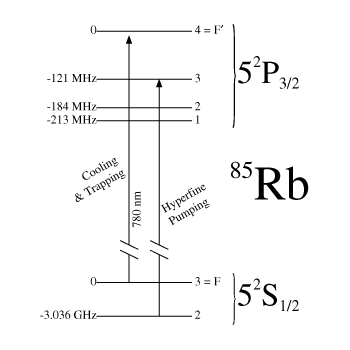
\includegraphics[width=0.6\textwidth]{images/transitions.png}
    \end{center}
    \caption{Diagram of the relevant transitions for rubidium-85~\cite{ust}}
\end{figure}
\subsection{Non-allowed and dark transitions}
\subsection{Saturated absorption spectroscopy}
\subsection{Doppler cooling}
\subsection{The Zeeman effect}
\subsection{Combined effects forming a MOT}
\subsection{Repumping}
\section{Experimental procedure}
\subsection{External-cavity diode lasers}
\subsection{Absorption spectroscopy}
\subsection{Saturated absorption spectroscopy}
\subsection{Vacuum cell setup}
\subsection{Magnetic quadrupole}
\subsection{Arrangement for optical molasses}
\subsection{Fine-tuning to create the trap}
\section{Results and discussion}
\vfill
\pagebreak
\section{References}
\bibliography{papers}
\bibliographystyle{unsrt}
\end{document}